\chapter{Objetivos}

En este proyecto el objetivo principal \textbf{OBJ-G} es desarrollar un dispositivo libre que permita monitorizar el consumo eléctrico tanto del hogar como de un dispositivo específico y que permita transmitir estos datos de forma inalámbrica, todo ello al menor precio posible.
Podemos dividir este objetivo principal en los siguientes objetivos principales:

\begin{itemize}
	\item\textbf{OBJ-P1} Diseño hardware con una placa que permita la conexión inalambrica WiFi para poder enviar los datos recogidos de un sensor no invasivo.
	
	\item\textbf{OBJ-P2} Implementación del firmware que permite capturar los datos que recoge el sensor y enviar estos datos vía WiFi.
	
	\item\textbf{OBJ-P3} Creación de un servidor web para poder almacenar los datos recibidos en una base de datos y que permitirá al usuario revisar consumos.
	
	\item\textbf{OBJ-P4} Documentación de todo el proyecto.
	
	
\end{itemize}

Una vez tenemos todos los objetivos principales definidos vamos a dividirlos en objetivos más específicos. Dentro de estos subobjetivos existirán algunos de ellos obligatorios para que la funcionalidad del proyecto sea completa y otros opcionales que servirán para perfeccionar el proyecto, pero estos no serán vitales para su correcto funcionamiento:

\begin{itemize}
	\item\textbf{OBJ-P1-OB1} Investigación de sensores de corriente no invasivos existentes en el mercado y como conectarlos a distintas placas.
	
	\item\textbf{OBJ-P1-OB2} Investigación para seleccionar la placa que mejor se adapte a este proyecto que cuente con conexión WiFi.
		
	
	\item\textbf{OBJ-P1-OB3} Montaje del primer prototipo con los componentes seleccionados anteriormente.
	
	\item\textbf{OBJ-P1-OP1} Mejora de este primer prototipo para añadir funcionalidades al proyecto.
	
	\item\textbf{OBJ-P1-OP2} Realizar todo el montaje de los componentes en un PCB para que el dispositivo tenga un buen acabado.
	
	\item\textbf{OBJ-P2-OB1} Decidir en que lenguaje programar la placa escogida y que IDE utilizar.
	
	\item\textbf{OBJ-P2-OB2} Implementar un primer firmware para asegurar que el hardware funciona adecuadamente.
	
	\item\textbf{OBJ-P2-OB3} Decidir en que formato y como se van a enviar las mediciones recogidas por la placa al servidor.
	
	\item\textbf{OBJ-P2-OP1} Mejorar el firmware para enviar más parámetros al servidor.
	
	\item\textbf{OBJ-P3-OB1} Selección de framework para crear la aplicación web.
	
	\item\textbf{OBJ-P3-OB2} Seleccionar el sistema de base de datos que vamos a utilizar para almacenar los datos recibidos por la placa.
	
	\item\textbf{OBJ-P3-OB3} Decidir donde alojar la base de datos y la aplicación web.
	
	\item\textbf{OBJ-P3-OB4} Implementar la aplicación web.
	
	\item\textbf{OBJ-P3-OP1} Mejorar la aplicación web para mostrar más información al usuario.
	
	\item\textbf{OBJ-P4-OB1} Subir a un repositorio de GitHub todo lo necesario para que las personas que estén interesadas puedan utilizar este proyecto por su cuenta de manera sencilla.
	
	\item\textbf{OBJ-P4-OB1} Realizar toda la documentación del proyecto en Latex siguiendo la plantilla ofrecida por la UGR.
	
	\item\textbf{OBJ-P4-OP1} Hacer un estudio de los consumos de algún electrodoméstico.
	
\end{itemize}

\section{Diagrama objetivos}

\begin{landscape}

	\begin{figure}
		\centering
		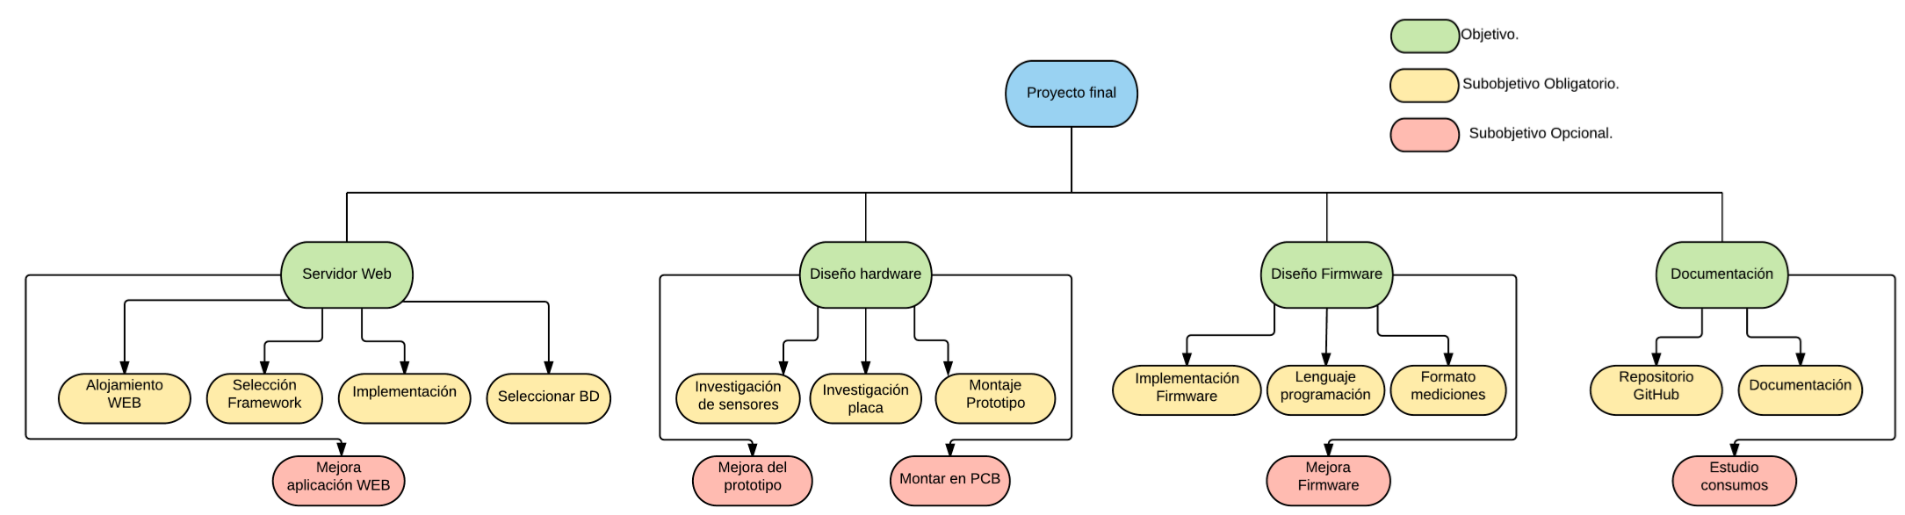
\includegraphics[scale=0.5]{imagenes/diagramaObjetivos.png}
		\caption{Diagrama de objetivos}
		\label{fig:Diagrama de objetivos}
	\end{figure}
	
\end{landscape}

\section{Conocimientos necesarios para alcanzar estos objetivos.}

Algunos de estos conocimientos han sido adquiridos tras cursar las asignaturas que se indicarán a continuación y otros de los conocimientos han sido adquiridos por mi propia cuenta al tener que realizar algunos de los objetivos de este proyecto:

\begin{itemize}
	\item\textbf{Conocimientos adquiridos mediante asignaturas de la carrera:}
	\begin{itemize}
		\item\textbf{Desarrollo de aplicaciones para internet:} Los conocimientos adquiridos tras cursar esta asignatura me han servido para poder realizar la web utilizando flask, además de conocer el lenguaje de programación python y las bases de datos NoSQL como MongoDB.
		\item\textbf{Infraestructura virtual:} Se han puesto en uso los conocimientos a la hora de utilizar git y GitHub.
		\item\textbf{Fundamentos de software:} Entre el temario de esta asignatura se encuentra una parte dedicada a la realización de scripts y algunos comandos básico de Linux que se han puesto en práctica para la realización de este proyecto.
		\item\textbf{Fundamentos de programación:} Donde se ven conceptos básicos sobre programación en c++ que en cierto modo han servido como base para realizar toda la parte de programación tanto web como a la hora de programar la placa.
	\end{itemize}
	\item\textbf{Conocimientos adquiridos gracias a la realización de este proyecto:}
		\begin{itemize}
		\item\textbf{\LaTeX:} He tenido que aprender Latex para poder realizar toda la documentación de este proyecto.
		\item\textbf{Arduino IDE:} A la hora de programar la placa he tenido que aprender como usar este IDE.
		\item\textbf{Electrónica básica:} Para poder llevar a cabo el montaje de todos los circuitos.
		\item\textbf{Raspberry Pi:} He necesitado adquirir conocimientos básicos para poder montar un servidor en una RaspberryPi.
		\item\textbf{Soldadura:} Conocimientos básicos de soldadura que nos permiten soldar pistas de estaño en la PCB para poder materializar los prototipos presentados en la protoboard en una placa real. 
		\item\textbf{Electricidad:} Necesario conocer un mínimo para poder calcular el Irms y la potencia ya que no tenia ningún tipo de conocimiento en este campo antes de realizar el proyecto.
	\end{itemize}
\end{itemize}



